\documentclass[12pt]{article}

\usepackage{sbc-template}
\usepackage{graphicx}
\usepackage{url}
\usepackage[utf8]{inputenc}
\usepackage[T1]{fontenc}
\usepackage[english, portuguese]{babel}
\usepackage{hyphenat}
\hyphenation{mate-mática recu-perar}
\usepackage{amsmath}
\usepackage{graphicx}
\graphicspath{ {imagens/} }
\usepackage{float}
\usepackage{environ}
\usepackage{graphicx}
\usepackage{subfigure}
\usepackage{booktabs}
\usepackage{multirow}

\NewEnviron{myequation}{%
\begin{equation}
\scalebox{1.5}{$\BODY$}
\end{equation}
}

\sloppy

\begin{document} 

\title{Avaliando a Influência da Modelagem Relacional e Colunar no Gerenciamento de Ambientes OLAP por meio do TPC-H}
\author{}
\address{}

\maketitle

\begin{abstract}

Companies have been using data warehouse (DW) environments and OLAP applications 
as decision making support. Due to data volume growth, more efficient ways to 
process them are needed. Relational DBMS are still widely used, however the NoSQL 
approach has been consolidating in market. To evaluate which one is the more appropriate 
in DW management, a comparative study between PostgreSQL and MonetDB DBMS is presented 
using TPC-H benchmark, under different data sizes. MonetDB was better among 
denormalized models and PostgreSQL at normalized ones. In general, MonetDB performed 
better than PostgreSQL.

\end{abstract}
     
\begin{resumo}
Empresas têm utilizado ambientes de data warehouse (DW) 
e aplicações OLAP como apoio à tomada de decisão. 
Devido ao crescimento do volume de dados, meios mais eficientes para o seu processamento 
são necessários. SGBD relacionais ainda são bastante utilizados para tal, 
porém a abordagem NoSQL também vêm se consolidando no mercado. 
Para avaliar qual é o mais apropriado no gerenciamento de DW, um estudo comparativo entre 
os SGBD PostgreSQL e o NoSQL MonetDB é aqui apresentado a 
partir do benchmark TPC-H, com diferentes volumes de dados. O MonetDB se 
destacou em modelagens mais denormalizadas e o PostgreSQL em modelagens normalizadas; e de maneira geral, 
o MonetDB obteve desempenho superior ao PostgreSQL.    
\end{resumo}

\section{Introdução}
Para tomar decisões de maneira rápida e inteligente Organizações têm como base os dados armazenados em seus repositórios.
Conforme o volume destes dados aumenta a má estruturação do repositório pode degradar o desempenho do acesso às informações,
e devido a isso a tecnologia de Data Warehouses (DW) é utilizada para persistência de dados e tomada de decisões de forma eficiente.

Além do armazenamento de dados, é necessário que se tenha uma aplicação que os acesse e traga informações
de maneira tão eficiente quanto à estruturação do repositório. Aplicações OLAP (\textit{Online Analytical Processing}) 
analisam dados multidimensionalmente 
e executam consultas analíticas, fazendo com que estejam fortemente associadas à DW.
Ao conjunto de DW e aplicações OLAP denomina-se ambiente OLAP.

Um ambiente OLAP deve ser projetado e implantado visando a rapidez na recuperação de dados \cite{wrembel2007data}, 
\cite{codd1998providing}, \cite{kimball2002dw}. Sistemas Gerenciadores de Bancos de Dados (SGBD) surgem como uma solução 
para esta questão, e duas classes de SGBD podem atuar como gerenciadores de DW, os relacionais e os NoSQL. 
Para que haja uma conclusão sobre qual abordagem é a melhor, a aplicação de um benchmark torna-se pertinente, 
e no escopo de banco de dados um benchmark que se destaca por tratar de sistemas de suporte à decisão é o TPC-H \cite{tpch2017page}. 

Outro fator que interfere no desempenho de um ambiente OLAP é a forma como este é modelado. 
Ambientes normalizados são utilizados pela facilidade de manutenção,
e o fácil entendimento acerca do relacionamento entre as entidades, que traz uma visão mais clara do sistema \cite{bax2003modelagem}. 
Entretanto, modelos denormalizados surgem para trazer ganho no desempenho das consultas, por diminuir 
as junções entre tabelas devido ao menor número de entidades.

Dadas estas condições, o objetivo aqui é realizar um estudo comparativo entre um SGBD relacional e outro NoSQL 
como gerenciadores de DW utilizando o TPC-H. Devido a seu amplo uso e poucas modificações na linguagem SQL, foi definido o PostgreSQL 
como SGBD relacional e o MonetDB como NoSQL, este por ainda utilizar SQL, possuir interface simples e ser o pioneiro 
entre os bancos NoSQL colunares.

\section{Recuperação e Persistência de Dados}

Um DW é definido como uma coleção de dados não-volátil, orientado ao assunto da organização, 
integrado e variante no tempo \cite{inmon2005building}. Ele é a base para todos os sistemas de 
suporte a decisão, atualmente definido como ambiente OLAP, e sua estrutura consiste de um 
repositório de dados homogêneo, local e centralizado \cite{wrembel2007data}.

É necessário que uma aplicação processe os dados contidos no repositório. DW trabalham sob uma grande 
massa de dados e executam consultas analíticas com base no suporte à decisão para acessar milhões de registros 
\cite{chaudhuri1997overview}, visando a união de dados com informações úteis para o mercado. Devido a isso, histórico, 
taxa de vazão de consultas e o tempo de resposta são fatores importantes ao processar os dados do DW.

Aplicações OLAP estão diretamente ligadas a DW pois seus objetivos englobam identificar tendências, 
padrões de comportamento e anomalias, e ainda relações entre dados \cite{codd1998providing} sob um grande 
volume de dados. Suas consultas são longas, consomem grande tempo de execução e estão interessadas em 
atributos específicos; e o processo de inserção de dados segue um processo conhecido como ETL (extração, transformação e carga), 
sendo mais complexo que pequenas transações \cite{vertabelo2017olap}. É neste processo que a modelagem conceitual do ambiente é definida. 
Ela tem como base a modelagem dimensional, ou multidimensional, fazendo uma analogia com um cubo para 
a representação de dados, uma vez que uma informação pode ser vista através de \textit{n} dimensões. 
Em sua concepção, a modelagem dimensional é composta por tabelas fato e tabelas dimensão.

Fatos representam regras ou métricas de negócio, e geralmente são descritos como atributos 
numéricos, relacionados à quantidades; ou aditivos, pois uma aplicação nunca irá retornar somente um fato, 
mas sim vários onde a operação mais recorrente é a soma de atributos.
Atributos textuais não definem um fato, na maioria das vezes apenas descrevem algo e são inseridos 
nas tabelas dimensão, que contem descrições a fim de tornar os fatos mais claros. Não é incomum encontrar tabelas dimensão  
com mais de 100 atributos e poucas tuplas, pois a intenção das dimensões é descrever as regras definidas por um 
fato. Nestas entidades são filtradas as consultas, compreendendo agrupamentos, padrões e ordenações, por exemplo.

Modelos dimensionais no escopo de um warehouse possuem apenas um fato com várias dimensões, fazendo com que 
sua estrutura se assemelhe a uma estrela, sendo conhecidos como modelos estrelas (\textit{star}). Este modelo é 
simples e torna eficiente a recuperação de dados por ter um número menor de junções. Entretanto, com a afirmação de 
que modelos normalizados são mais fáceis para se dar manutenção, alguns modelos \textit{star} podem ser trabalhados 
criando-se novas tabelas denominadas subdimensão. Estes modelos caracterizam modelagens relacionais e são conhecidos 
como modelos \textit{snowflake}.

Para comparar o desempenho entre modelagens pode-se utilizar SGBD como gerenciadores de DW.
Eles possuem algumas vantagens que os tornam úteis para tal, como controle de redundância, restrições de acesso, 
inserção de índices, restrições de integridade, possibilidade de realizar backup e restauração de dados, e persistência 
de dados garantida. Um modelo de SGBD muito conhecido e utilizado é o relacional. Esta classe está atrelada à dados 
mais normalizados por seguir a tradicional modelagem relacional, fazendo com que se aproxime do modelo \textit{snowflake} de DW; 
e ainda preza pelos conceitos de ACID. Modelos 
assim definidos possuem algumas limitações quanto à escalabilidade, complexidade e o fato de todas as informações serem 
mantidas e recuperadas sob a forma de tuplas \cite{leavitt2010will}. Tais limitações podem degradar o desempenho de 
um ambiente analítico, visto que uma consulta analítica processa apenas os atributos necessários. Mesmo a adição de 
índices não ajudaria, devido a necessidade de ler estes índices \cite{matei2010column}. Para suprir estes problemas 
SGBD NoSQL podem ser utilizados.

O fortalecimento do movimento NoSQL se deu em 2007 com um artigo da Amazon sobre o banco Dynamo 
\cite{decandia2007dynamo, leavitt2010will}, cujo objetivo era satisfazer algumas deficiências apontadas 
pelos SGBD relacionais, para tanto trabalham com modelagens de dados mais denormalizadas e podem ser classificados 
de diferentes formas de acordo com sua estruturação. Também, NoSQL tendem a não se ater ao ACID e optar por disponibilidade e particionamento 
de acordo com o teorema CAP \cite{brewer2000towards} para realizar operações de forma mais rápida e possibilitar escalabilidade. 
O banco NoSQL que melhor trabalha ainda com a linguagem SQL é o modelo colunar. Seu 
diferencial é o armazenamento de todas as instâncias de um mesmo atributo junto. Isto reduz o tempo de acesso e 
escrita em disco \cite{matei2010column, abadi2008query}, retornando apenas os atributos solicitados; e também 
torna possível a compressão de dados \cite{abadi2006integrating} e a eficiência em operações 
matemáticas de agregação \cite{matei2010column}.

\section{TPC-H}
Para selecionar qual SGBD é o mais adequado a cada modelagem em ambientes OLAP a 
realização de um benchmark é o mais indicado. De acordo com seu manual de especificação \cite{tpc2017specs}, o TPC-H 
é um benchmark de suporte à decisão de negócios, representando grandes volumes de dados e executando 
consultas com um alto grau de complexidade a fim de responder questões críticas de negócio. Ele propõe 
uma modelagem \textit{snowflake} que pode ser encontrada no manual do TPC-H \cite{tpc2017specs}.

O TPC-H não apresenta uma modelagem denormalizada de dados similar à \textit{star}. Para tanto, foi construído 
um ambiente denormalizado a partir do ambiente original do TPC-H para as devidas comparações. 
Essa construção se fundamentou na criação de um modelo com 
uma única entidade fato central, unindo atributos de diferentes fatos, descrita por dimensões; e 
na remoção de tabelas subdimensão.

Cada SGBD é executado sobre os dois ambientes, \textit{snowflake} e \textit{star}.
Em cada ambiente será executado o teste de desempenho, que é composto de duas execuções: 
o teste de força e o teste de vazão. Estas duas execuções são utilizadas para calcular o 
desempenho do SGBD, utilizando a unidade de medida \textit{QphH@Size}, que corresponde à quantidade 
de consultas executadas por hora para determinado tamanho de banco de dados.

O primeiro teste, de força, mede a taxa de consultas por hora do sistema com um único usuário ativo. 
Neste teste são executadas em uma única sessão três instruções: inserção de novos registros, consultas 
em SQL para recuperar informações, e remoção da mesma quantia de registros inseridos; exatamente nesta ordem. O 
segundo, o teste de vazão, mede a capacidade do sistema de processar a maior quantidade de consultas no menor 
intervalo de tempo. Sua execução se dá sob um número mínimo de sessões, também de acordo com o tamanho 
da base. É criada uma sessão para executar a inserção e remoção de dados, e \textit{n} sessões para as consultas ao 
banco; sendo estas instruções executadas concorrentemente.

\section{O Experimento}

O estudo foi feito para bases de diferentes tamanhos, sendo estes de 1GB, 10GB e 30GB. Previamente foi analisado 
também o tempo para realizar a carga de dados nos SGBD. Logo ao analisar os resultados notou-se que uma base 
denormalizada leva mais tempo para o carregamento. Isto deve-se à redundância de dados de alguns atributos que 
antes eram tratados em entidades separadas, aumentando o tamanho das entidades das quais eles agora fazem parte.

O processo do TPC-H foi desenvolvido utilizando o driver JDBC devido a simplificação 
que seu uso traz ao desenvolvimento de aplicações e por dar suporte à vários SGBD. A 
execução começa com o teste de força seguido do teste de vazão, e estas execuções já 
mostram diferenças entre os SGBD, como visto na Tabela \ref{tab:power-vazao-normalizado}. O teste de força 
mostrou-se superior para todas as bases de dados, porém o teste de vazão, que testa 
como se comporta o sistema com mais de um usuário ativo através de execuções paralelas, 
apresenta comportamento diferente conforme a base aumenta, evidenciando um desempenho 
melhor do PostgreSQL sob o MonetDB.

\begin{table}[htpb]
    \centering
    \caption{Valores dos testes de força e vazão para os cenários normalizados de teste}
    \label{tab:power-vazao-normalizado}
    \begin{tabular}{c|ccc|c}
    \hline
    \multirow{2}{*}{SGBD} & \multicolumn{3}{c|}{Base de Dados (GB)} & \multirow{2}{*}{Execução}       \\
                          & 1             & 10         & 30         &                                 \\ \hline
    MonetDB               & 4.231         & 7.237      & 4.292      & \multirow{2}{*}{Teste de Força} \\
    PostgreSQL            & 2.022         & 1.120      & 0.781      &                                 \\ \hline
    MonetDB               & 1622.929      & 3.305      & 0.125      & \multirow{2}{*}{Teste de Vazão} \\
    PostgreSQL            & 958.028       & 3.645      & 0.244      &                                 \\ \hline
    \end{tabular}
\end{table}

Ao contrário do cenário normalizado, no denormalizado o MonetDB obteve valores 
superiores ao PostgreSQL em ambos os testes, conforme a Tabela \ref{tab:power-vazao-denormalizado} 
evidenciando que o MonetDB em ambiente denormalizado consegue ter ganhos 
ao normalizado para paralelismo; apesar disso algumas consultas do teste de força 
adaptadas do ambiente original do TPC-H demoraram mais que as originais, fazendo com que 
os resultados do normalizado sejam um pouco melhores ao denormalizado.

\begin{table}[htpb]
    \centering
    \caption{Valores dos testes de força e vazão para os cenários denormalizados de teste}
    \label{tab:power-vazao-denormalizado}
    \begin{tabular}{c|ccc|c}
    \hline
    \multirow{2}{*}{SGBD} & \multicolumn{3}{c|}{Base de Dados (GB)} & \multirow{2}{*}{Execução}       \\
                          & 1             & 10         & 30         &                                 \\ \hline
    MonetDB               & 3.435         & 4.643      & 3.253      & \multirow{2}{*}{Teste de Força} \\
    PostgreSQL            & 1.291         & 0.355      & 0.302      &                                 \\ \hline
    MonetDB               & 2468.020      & 5.836      & 0.184      & \multirow{2}{*}{Teste de Vazão} \\
    PostgreSQL            & 637.310       & 1.495      & 0.134      &                                 \\ \hline
    \end{tabular}
    \end{table}

Tendo os valores de execução dos testes de força e vazão, estes foram aplicados 
no cálculo de desempenho final para o benchmarking. Analisando os ambientes isoladamente 
o MonetDB destacou-se na modelagem \textit{star} por ser mais denormalizada, com 
ganhos de 11.11\%, 6.43\% e 5.53\% para as bases de 1, 10 e 30GB.  
O PostgreSQL por ser um SGBD relacional teve destaque no ambiente \textit{snowflake}, 
com ganhos de 53.44\%, 177.39\% e 117.32\% para as mesmas bases. 
As Figuras \ref{fig:qph_monet} e \ref{fig:qph_psql} ilustram os resultados graficamente 
em conjunto de seus valores para o MonetDB e o PostgreSQL, respectivamente. 

\begin{figure*}[htpb]
    \centering
    \subfigure[]{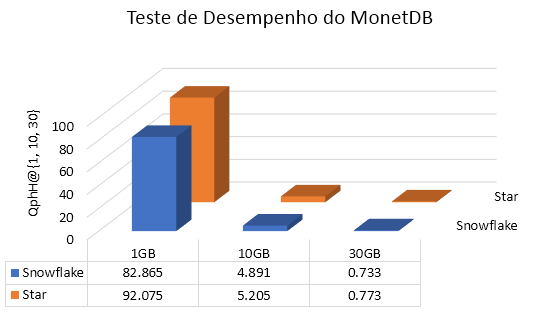
\includegraphics[width=7.2cm]{qph_monetdb}\label{fig:qph_monet}}
    \subfigure[]{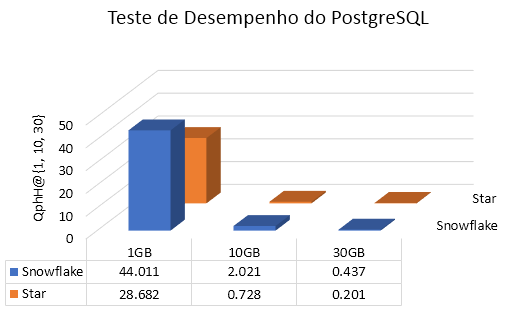
\includegraphics[width=7.2cm]{qph_postgres}\label{fig:qph_psql}}
    \caption{Ilustração dos resultados entre os SGBD}\label{fig:qph_sgbd}
\end{figure*}

Tomando como base os ambientes e comparando os SGBD, o MonetDB obteve ganhos sob o PostgreSQL 
em todos os cenários. Este resultado era esperado se levar em conta o armazenamento 
e leitura aprimorados do MonetDB, apesar dos resultados apresentados pelo teste de força. 
Os ganhos para as respectivas bases foram de 88.29\%, 142.04\% e 67.66\% no ambiente 
normalizado e 221.02\%, 614.57\% e 284.51\% no ambiente denormalizado.

\begin{figure*}[htpb]
    \centering
    \subfigure[]{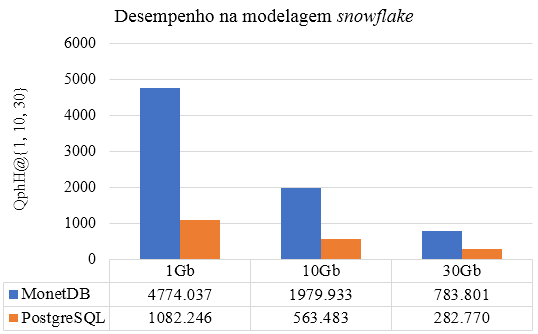
\includegraphics[width=7.2cm]{qph_snowflake}\label{fig:qph_snowflake}}
    \subfigure[]{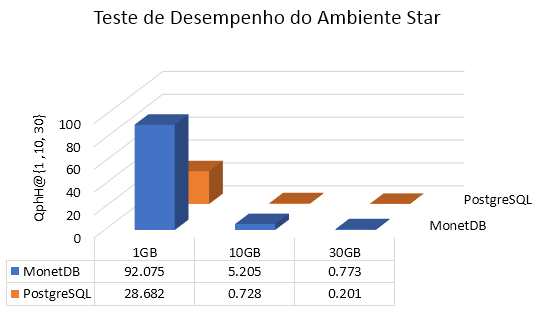
\includegraphics[width=7.2cm]{qph_star}\label{fig:qph_star}}
    \caption{Ilustração dos resultados entre os ambientes}\label{fig:qph_ambiente}
\end{figure*}

\section{Conclusão e Trabalhos Futuros}

Com alguns ganhos superiores à 100\% no ambiente normalizado e todos superiores à 
200\% no denormalizado com seu melhor valor sendo 7 vezes melhor que o do PostgreSQL, 
corrobora-se a ideia de que um SGBD NoSQL pode trazer vantagens para ambientes OLAP, 
por adaptar-se melhor à modelagem comumente utilizada por DW. Embora algumas consultas 
do ambiente denormalizado tenham levado um pouco mais de tempo para executar isso não 
interferiu de maneira crítica no benchmark.

Como continuidade para o projeto, propõe-se a inclusão de mais SGBD NoSQL de 
diferentes classes para que possa analisar se a mudança na estruturação de SGBD 
que não utilizam SQL para manipulação do banco tem impacto direto em ambientes empresariais. 
Exemplos destes são o MongoDB e o Neo4J, que possuem linguagem orientada a documento e 
grafo, respectivamente. Ainda, será realizada a aplicação dos resultados do estudo em 
empresas que utilizam uma modelagem relacional juntamente com SGBD relacionais, a fim 
de verificar se a mudança para um NoSQL sob modelagem denormalizada irá trazer 
vantagens à empresa.

\bibliographystyle{sbc}
\bibliography{REFERENCES}

\end{document}
